\documentclass[11pt,a4paper]{article}

% === PACKAGES ===
\usepackage[utf8]{inputenc}
\usepackage[T1]{fontenc}
\usepackage{amsmath,amssymb,amsfonts}
\usepackage{booktabs}
\usepackage{graphicx}
\usepackage{hyperref}
\usepackage[margin=2.5cm]{geometry}
\usepackage{xcolor}
\usepackage{multirow}
\usepackage{textcomp}
\usepackage{array}
\usepackage{caption}
\usepackage{float}

% === FIGURE PATH (for arXiv / out-of-tree builds) ===
\graphicspath{{./}{../figures/}}

% === HYPERREF SETUP ===
\hypersetup{
  colorlinks=true,
  linkcolor=blue!60!black,
  citecolor=blue!60!black,
  urlcolor=blue!60!black
}

% === CUSTOM COMMANDS ===
\newcommand{\pval}[1]{\ensuremath{p = #1}}

% === TITLE ===
\title{%
  Statistical evidence for golden ratio structure\\
  in elementary fermion mass ratios\\
  with QCD regime dependence%
}

\author{%
  M.\ Tromel\thanks{Corresponding author. E-mail: marc.troe@gmail.com.
  ORCID: \href{https://orcid.org/0009-0005-9229-3502}{0009-0005-9229-3502}}\\[4pt]
  \textit{Independent Researcher, N\"urtingen, Germany}
}

\date{March 2026}

\begin{document}
\maketitle

% ============================================================
% ABSTRACT
% ============================================================
\begin{abstract}
We report a statistically significant golden ratio
($\Phi = (1{+}\sqrt{5})/2 \approx 1.618$) structure in the mass ratios
of elementary fermions. Starting from the electron mass alone, a
recursive bootstrap algorithm reproduces 11 Standard Model particle
masses using five $\Phi$-based operators, with a mean error of 2.5\%.
The operator exponents $\{3, 4, 11\}$ are Lucas numbers ($L_2, L_3, L_5$),
and the non-integer operators $\Phi^\Phi$ and $\Phi^{1/\Phi}$ satisfy
$\Phi^\Phi / \Phi^{1/\Phi} = \Phi$ (proven from $\Phi^2 = \Phi + 1$).
A universality test shows no alternative constant
$K \in [1.2,\, 2.5]$ describes all five core relations simultaneously
with integer exponents ($p = 0.001$). A basis scan over 500 alternatives confirms that
among standard mathematical constants, only $\Phi$ achieves full
reproduction at 10\% tolerance ($e$: 1/11, $\pi$: 1/11, base~2: 9/11);
all successful bases in the scan are powers of~$\Phi$.
The six independent $\Phi$-ladders
defined by nine fermion masses are significantly uniformly distributed
(Greenwood test, $p = 0.007$). Chain connectivity at 5\% tolerance is
highly significant ($p = 0.006$) and strengthens at tighter tolerance.
In the hadron spectrum, $\Phi$-relations manifest exclusively in the
QCD-dominated regime (binding energy $> 50\%$ of hadron mass): Fisher
exact test yields $p = 0.008$ with perfect separation (4/4 vs.\ 0/5).
A holdout test over 167 PDG hadrons finds no statistically significant
$\Phi$-grid proximity ($p = 0.055$, one-sided; $p = 0.91$ with conservative
4-seed subset), and gauge bosons show no $\Phi$-signal (all $p > 0.5$).
Three specific hadron relations in the light QCD regime survive all
controls (Fisher combined $p = 2.2 \times 10^{-5}$). All results are reproducible
via companion code.
\end{abstract}

\noindent\textbf{Keywords:}
fermion masses, golden ratio, mass relations, Lucas numbers,
QCD regime dependence, hadron spectrum, statistical test

% ============================================================
% 1. INTRODUCTION
% ============================================================
\section{Introduction}
\label{sec:intro}

The Standard Model of particle physics contains 15 Yukawa coupling
constants that determine the masses of the elementary fermions
(6 quarks, 3 charged leptons, and at least 2 massive neutrinos).
These parameters are not predicted by the theory; they are extracted
from experiment and span more than five orders of magnitude, from
$m_e = 0.511$~MeV to $m_t = 172{,}760$~MeV. Whether an organizing
principle underlies these apparently arbitrary values remains one of
the central open questions in particle physics~\cite{Xing2020,Fritzsch2000}.

Several empirical mass relations have been proposed. Nambu~\cite{Nambu1952}
observed that particle masses are approximately quantized in units of
$m_e / \alpha \approx 70$~MeV, where $\alpha$ is the fine structure
constant. Barut~\cite{Barut1979} proposed a lepton mass formula
based on $\alpha^{-1} n^4$ scaling. MacGregor~\cite{MacGregor2007}
systematized these observations as ``$\alpha$-quantization.'' The most
prominent is the Koide formula~\cite{Koide1982}, which relates the
three charged lepton masses through the surprisingly precise identity
\begin{equation}
  \frac{m_e + m_\mu + m_\tau}
       {\bigl(\sqrt{m_e} + \sqrt{m_\mu} + \sqrt{m_\tau}\bigr)^2}
  = \frac{2}{3}\,,
  \label{eq:koide}
\end{equation}
satisfied to better than 0.01\%. Despite extensive theoretical
work~\cite{Sumino2009,GaoLi2016,Sun2021,RiveroGsponer2005,Foot1994},
the physical
origin of this relation remains unexplained. Extensions to the quark
sector show approximate validity~\cite{GaoLi2016}.

In the present work, we report a different class of mass relations
based on the golden ratio $\Phi = (1{+}\sqrt{5})/2 \approx 1.618$.
The golden ratio has appeared in condensed matter physics as an
emergent symmetry ratio in quantum critical Ising
chains~\cite{Coldea2010}; its appearance in the particle mass
spectrum has not been systematically investigated before.
We perform a systematic statistical analysis, including falsification
tests, negative controls, and a regime-dependent analysis of the
hadron spectrum.

\textbf{We emphasize that this paper reports an empirical observation
with rigorous statistical evaluation, not a new theory.} We do not
claim to explain \emph{why} $\Phi$ appears; we demonstrate
\emph{that} it appears, quantify the statistical significance,
delineate the domain of validity, and present falsifiable predictions.

% ============================================================
% 2. THE PHI CHAIN
% ============================================================
\section{The \texorpdfstring{$\Phi$}{Phi}-chain: fermion masses from the electron}
\label{sec:chain}

\subsection{Mass spectrum}
\label{sec:spectrum}

Starting from the electron mass $m_e = 0.511$~MeV as the sole input,
we construct a correlation graph in which each particle mass is
related to a ``parent'' mass by one of five $\Phi$-operators or by a
geometric mean (impedance) of two already-identified masses. The
algorithm is defined in Appendix~\ref{app:algorithm}.

Table~\ref{tab:genesis} shows the resulting predictions against
PDG~2024 reference values~\cite{PDG2024}. Each row represents a
single algebraic relation: the predicted mass is computed from the
PDG value of the parent particle.

\begin{table}[H]
\centering
\caption{Genesis predictions vs.\ PDG~2024 reference masses.
Each prediction uses the PDG mass of the parent particle.
$\Phi = (1{+}\sqrt{5})/2 = 1.6180339887\ldots$}
\label{tab:genesis}
\begin{tabular}{@{}lrrcr@{}}
\toprule
Particle & $M_\text{pred}$ (MeV) & $M_\text{PDG}$ (MeV) &
  Relation & Error \\
\midrule
Electron & 0.511 & 0.511 & Seed & --- \\
Up       & 2.165  & 2.16  & $m_e \times \Phi^3$          & 0.2\% \\
Down     & 4.714  & 4.67  & $m_u \times \Phi^\Phi$       & 0.8\% \\
Strange  & 95.02  & 93.4  & $\sqrt{m_u \cdot m_b}$       & 1.7\% \\
Muon     & 101.69 & 105.66 & $m_e \times \Phi^{11}$      & 3.8\% \\
Pion     & 139.72 & 139.57 & $\sqrt{m_d \cdot m_b}$      & 0.1\% \\
Proton   & 956.6  & 938.3  & $m_\pi \times \Phi^4$       & 2.0\% \\
Charm    & 1{,}263 & 1{,}270 & $m_p \times \Phi^{1/\Phi}$ & 0.5\% \\
Tau      & 1{,}710 & 1{,}777 & $m_c \times \Phi^{1/\Phi}$ & 3.8\% \\
Bottom   & 4{,}017 & 4{,}180 & $\sqrt{m_s \cdot m_t}$     & 3.9\% \\
Top      & 186{,}721 & 172{,}760 & $m_p \times \Phi^{11}$ & 8.1\% \\
\midrule
\multicolumn{4}{l}{Mean error (10 non-seed particles)} & 2.5\% \\
\multicolumn{4}{l}{Median error} & 1.8\% \\
\bottomrule
\end{tabular}
\end{table}

\noindent
Figure~\ref{fig:pred_vs_obs} shows the predictions on a log--log scale.

\begin{figure}[H]
\centering
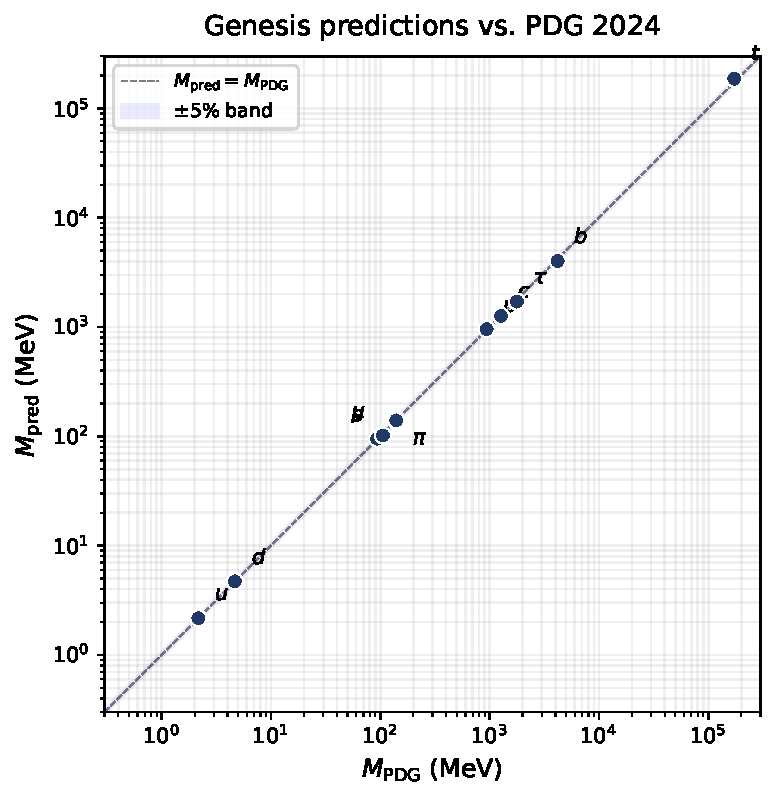
\includegraphics[width=0.75\textwidth]{fig1_pred_vs_obs.pdf}
\caption{Genesis predictions vs.\ PDG~2024 masses on a log--log scale.
The dashed line indicates perfect agreement; the shaded band shows
$\pm 5\%$. All 10 non-seed particles fall within 8.1\% of the
diagonal.}
\label{fig:pred_vs_obs}
\end{figure}

\noindent
\textbf{Note on mass conventions.}
The reference masses follow the PDG standard~\cite{PDG2024}: pole masses for leptons
and the top quark,\footnote{We use $m_t = 172{,}760$~MeV following the
PDG~2020 world average. The PDG~2024 update gives
$172{,}570 \pm 290$~MeV; substituting this value shifts the mean Genesis
error by less than 0.02 percentage points and leaves all statistical
conclusions unchanged.} $\overline{\text{MS}}$ at $\mu = 2$~GeV for light
quarks ($u$, $d$, $s$), $\overline{\text{MS}}$ at $\mu = m_q$ for
charm and bottom, and physical masses for pion and proton. Four of the
eleven chain entries depend on this convention; a convention-independent
subset is tested separately in Section~\ref{sec:convindep}.

\subsection{Algebraic structure of the operators}
\label{sec:algebra}

The five operators $\{\Phi^3, \Phi^4, \Phi^{11}, \Phi^\Phi,
\Phi^{1/\Phi}\}$ possess nontrivial algebraic properties:

\paragraph{Non-integer operators.}
The identity
\begin{equation}
  \frac{\Phi^\Phi}{\Phi^{1/\Phi}}
  = \Phi^{\,\Phi - 1/\Phi}
  = \Phi^1
  = \Phi
  \label{eq:selfref}
\end{equation}
follows directly from $\Phi^2 = \Phi + 1$:
\begin{equation}
  \Phi - \frac{1}{\Phi}
  = \frac{\Phi^2 - 1}{\Phi}
  = \frac{(\Phi + 1) - 1}{\Phi}
  = 1\,.
  \label{eq:selfref_proof}
\end{equation}
This is an exact algebraic identity, not a numerical approximation.
The two non-integer operators contribute zero free parameters.

\paragraph{Integer exponents and Lucas numbers.}
The exponents $\{3, 4, 11\}$ are Lucas numbers~\cite{Koshy2001}:
$L_2 = 3$, $L_3 = 4$, $L_5 = 11$, where the Lucas sequence is
defined by $L_0 = 2$, $L_1 = 1$, $L_n = L_{n-1} + L_{n-2}$.
(Note: these are not consecutive Lucas numbers; $L_4 = 7$ is absent.)
Lucas numbers satisfy $\text{round}(\Phi^n) = L_n$ for $n \geq 2$,
i.e., they are the nearest-integer approximation of $\Phi$-powers.
Notably, 4 and 11 are \emph{not} Fibonacci numbers; only the Lucas
sequence contains all three exponents.

\paragraph{Free parameters.}
Given the algebraic constraints above, the five operators contain zero
free exponents. \emph{Qualification:} structural degrees of freedom
remain --- specifically the target set, mass definitions, the 20\%
matching tolerance, and the search rules. These are documented in
Appendix~\ref{app:algorithm}.

% ============================================================
% 3. STATISTICAL TESTS
% ============================================================
\section{Statistical validation}
\label{sec:stats}

\subsection{\texorpdfstring{$\Phi$}{Phi}-universality test}
\label{sec:universality}

\textbf{Question:} Is there an alternative constant $K \neq \Phi$
that simultaneously describes all core relations with integer
exponents?

For each of five independent mass ratios (Table~\ref{tab:universality}),
we compute the $\Phi$-exponent
$n = \log(\text{ratio})/\log(\Phi)$ and its distance to the nearest
integer, $\Delta n = |n - \text{round}(n)|$.

\begin{table}[H]
\centering
\caption{Five core mass relations and their $\Phi$-exponents.}
\label{tab:universality}
\begin{tabular}{@{}lcccc@{}}
\toprule
Relation & Mass ratio & $n_\Phi$ & $\text{round}(n)$ & $\Delta n$ \\
\midrule
$m_u / m_e$                        & 4.227  & 2.996  & 3  & 0.004 \\
$m_\mu / m_e$                      & 206.77 & 11.080 & 11 & 0.080 \\
$m_\tau / m_e$                     & 3{,}477.2 & 16.945 & 17 & 0.055 \\
$M_{\Omega^-} / m_s$               & 17.906 & 5.996  & 6  & 0.004 \\
$\Delta M_\text{dec} / \Delta m_q$ & 1.632  & 1.017  & 1  & 0.017 \\
\bottomrule
\end{tabular}
\end{table}

\noindent
The observed maximum is
$\max|\Delta n|(\Phi) = 0.080$ (muon--electron ratio).

\textbf{Monte Carlo test:}
We draw $2 \times 10^5$ random constants $K$ uniformly in $[1.2, 2.5]$.
For each $K$, we compute $\max|\Delta n|(K)$ over all five relations.

\textbf{Result:}
$P\bigl(\max|\Delta n|(K) \leq 0.080\bigr) = 0.0009$.
Fewer than 1\textperthousand{} of constants describe all five relations as
well as $\Phi$ (Figure~\ref{fig:universality}).

\begin{figure}[H]
\centering
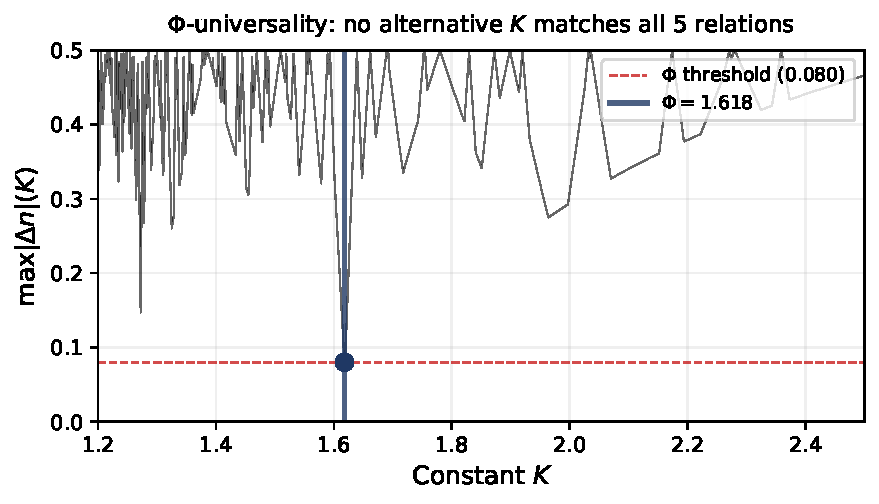
\includegraphics[width=0.85\textwidth]{fig2_universality.pdf}
\caption{$\Phi$-universality test: the maximum deviation
$\max|\Delta n|(K)$ over five core mass relations, scanned across
constants $K \in [1.2, 2.5]$. The golden ratio (vertical line,
$\Phi = 1.618$) achieves the joint minimum. No other constant below
the dashed threshold exists in the scanned range.}
\label{fig:universality}
\end{figure}

\subsection{Phase uniformity of \texorpdfstring{$\Phi$}{Phi}-ladders}
\label{sec:phase}

Each fermion mass $m$ defines a $\Phi$-phase
$\phi = \{\log(m/m_e)/\log\Phi\} \in [0,1)$, where $\{x\}$ denotes
the fractional part. Particles with similar phase ($|\Delta\phi| < 0.08$,
circular distance) belong to the same $\Phi$-ladder.

The nine elementary fermion masses form six independent ladders
(Table~\ref{tab:ladders}). Their phases are tested for uniformity on
the circle $[0,1)$ using the Greenwood statistic
$G = \sum_i g_i^2$, where $g_i$ are the circular gaps between
adjacent ladder phases~\cite{Greenwood1946,FisherCircular1993}.

\begin{table}[H]
\centering
\caption{Six $\Phi$-ladders from nine elementary fermion masses.}
\label{tab:ladders}
\begin{tabular}{@{}clc@{}}
\toprule
Ladder & Members & Phase (circular mean) \\
\midrule
1 & $e$, $u$, $\mu$, $\tau$ & 0.005 \\
2 & $c$                      & 0.247 \\
3 & $t$                      & 0.456 \\
4 & $d$                      & 0.598 \\
5 & $b$                      & 0.722 \\
6 & $s$                      & 0.823 \\
\bottomrule
\end{tabular}
\end{table}

\noindent
\textbf{Result:}
$G_\text{obs} = 0.181$ vs.\ $G_\text{expected} = 1/6 = 0.167$.
Monte Carlo ($5 \times 10^5$ random configurations of 6 points on
$[0,1)$): $P(G \leq G_\text{obs}) = 0.007$.

The six ladders are distributed more uniformly than 99.3\% of random
configurations. The $\Phi$-lattice tiles the logarithmic mass space
systematically, not randomly.

\subsection{Chain connectivity}
\label{sec:connectivity}

\textbf{Question:} How unusual is the real particle spectrum's
connectivity under $\Phi$-operators?

Starting from the seed (electron), we attempt to reach all 11 target
masses through single operator applications or pairwise geometric
means (impedances). We compare against $5{,}000$ pseudo-spectra
(11 masses drawn log-uniformly in $[m_e, m_t]$); results are shown
in Table~\ref{tab:connectivity}.

\begin{table}[H]
\centering
\caption{Chain connectivity: real spectrum vs.\ pseudo-spectra.}
\label{tab:connectivity}
\begin{tabular}{@{}cccc@{}}
\toprule
Tolerance & Real ($\Phi$) & Pseudo (mean) & $p$-value \\
\midrule
10\% & 11/11 & 3.8/11 & 0.066 \\
\textbf{5\%}  & \textbf{10/11} & 1.8/11 & \textbf{0.006} \\
\textbf{3\%}  & \textbf{7/11}  & 1.4/11 & \textbf{0.005} \\
\bottomrule
\end{tabular}
\end{table}

\noindent
The signal \emph{strengthens} at tighter tolerance --- the opposite
of a geometric coverage artifact. At 10\% tolerance, random spectra
occasionally achieve connectivity by chance. At 3\%, chance connections
vanish but the real signal persists. This is the qualitative
fingerprint of structure versus noise.

\subsection{Convention-independent subset}
\label{sec:convindep}

Seven of the eleven particles use only pole masses or physical masses
that do not depend on a renormalization convention: $e$, $\mu$, $\tau$,
pion, proton, bottom ($\overline{\text{MS}}$ at $m_b$, i.e.,
self-scale), and top.

For this seven-particle subset: chain connectivity at 5\% yields
$p = 0.014$; a basis scan over 300 random bases $\beta \in [1.05, 3.5]$
gives $\Phi$ rank \#2/300 ($p = 0.007$). The signal exists
independently of the 2~GeV convention.

\subsection{Robustness: alternative bases and tolerances}
\label{sec:robustness}

A systematic scan over 500 equally spaced bases
$\beta \in [1.05, 3.5]$ shows that 56 bases (11.2\%) reproduce
all 11 particles at 20\% tolerance. These bases cluster in five
groups, all centered at powers of~$\Phi$: near $\Phi \approx 1.62$
(12~bases), $\Phi^{1.4} \approx 2.0$ (15~bases),
$\Phi^{1.9} \approx 2.5$ (7~bases),
$\Phi^{2.4} \approx 3.2$ (20~bases), and $\Phi^{0.7} \approx 1.4$
(2~bases). No non-$\Phi$-related region achieves full reproduction.
At 10\% tolerance, only two clusters survive: the $\Phi$-neighborhood
(4~bases) and its reparametrization $\Phi^{2.4}$ (6~bases); at 5\%,
no base achieves 11/11.

Crucially, the $\Phi$-cluster separates from all alternatives at
reduced tolerance (Table~\ref{tab:tol_sensitivity}):

\begin{table}[h]
\centering
\caption{Number of particles reproduced (out of 11) by the Genesis
algorithm for different bases and tolerances.}
\label{tab:tol_sensitivity}
\begin{tabular}{@{}ccccc@{}}
\toprule
Tolerance & $\Phi$ (1.618) & $e$ (2.718) & $\pi$ (3.142) & 2 \\
\midrule
5\%  & 10/11 & 1/11 & 1/11 & 1/11 \\
\textbf{10\%} & \textbf{11/11} & 1/11 & 1/11 & 9/11 \\
15\% & 11/11 & 1/11 & 10/11 & 11/11 \\
20\% & 11/11 & 1/11 & 11/11 & 11/11 \\
\bottomrule
\end{tabular}
\end{table}

\noindent
At 10\% tolerance, $\Phi$ is the \emph{only} standard mathematical constant
that achieves complete reproduction. The Euler number $e$ never finds
more than the seed electron; $\pi$ reaches only 1/11 at 10\% but
achieves 10/11 at 15\% through the $\Phi^{2.4}$ reparametrization
channel (since $\pi \approx 3.14$ lies near $\Phi^{2.4} \approx 3.19$).
The base~2 requires $\geq 10\%$ tolerance (9/11) and reaches 11/11 at
15\%. The secondary cluster at $\beta \approx 3.19 \approx \Phi^{2.4}$
that also achieves 11/11 at 10\% is a reparametrization, not an
independent constant: it exists because $\beta^{11} \approx m_t/m_e$,
exploiting the same $\Phi$-structured mass ratios through rescaled
exponents. This asymmetry is the strongest single argument against
a ``numerology'' interpretation: it shows that $\Phi$ is not
interchangeable with other irrational constants.

\subsection{PDG measurement uncertainties}
\label{sec:pdg_errors}

PDG measurement uncertainties range from $< 10^{-6}$ (electron,
muon) to 3.2\% (up quark). For 8 of 11 particles, the relative
experimental uncertainty is below 1\%, i.e., one to two orders of
magnitude smaller than the typical Genesis deviation (2.5\% mean).
Sensitivity to PDG measurement uncertainties varies across tests and
is governed by which input masses carry large relative errors.
The lepton masses ($m_e$, $m_\mu$, $m_\tau$) are known to
$< 10^{-5}$ relative precision, so any test depending only on leptons
is insensitive to measurement uncertainties.
Tests involving light quark masses, however, inherit the large
$\overline{\text{MS}}$ uncertainties:
$m_u = 2.16^{+0.49}_{-0.26}$~MeV ($\sim 20\%$) and
$m_s = 93.4^{+8.6}_{-3.4}$~MeV ($\sim 6\%$).
A systematic $\pm 1\sigma$ perturbation analysis ($5 \times 10^5$
Monte Carlo trials per configuration; code in companion repository)
shows the following:

\begin{itemize}
  \item \textbf{Robust} ($p$-value shift $< 0.01$):
        $m_\mu/m_e \approx \Phi^{11}$ and $m_\tau/m_e \approx \Phi^{17}$
        (lepton sub-chain), A4 regime hypothesis (binary classification
        insensitive to quark mass shifts), B3 $b$-replacement
        (depends only on $\tau$ and directly measured hadron masses).
  \item \textbf{Moderately sensitive} ($p$-value shift $\lesssim 0.1$):
        A2 Greenwood test (cluster composition and gap structure
        shift when $m_s$ moves by $1\sigma$, potentially changing
        the number of effective ladders), B1 $\Omega^-$ prediction
        (degraded by factor~42 in $\Delta n$ at $m_s + 1\sigma$).
  \item \textbf{Strongly sensitive}:
        A1 Genesis chain ($m_u/m_e \approx \Phi^3$ degrades from
        $\Delta n = 0.004$ to $0.42$ at $m_u + 1\sigma$),
        A3 $\Phi$-universality ($p$ shifts from $0.001$ to $0.4$ at
        $m_u + 1\sigma$), B2 decuplet amplification ($8\%$ deviation
        from $\Phi$ at $m_s + 1\sigma$).
\end{itemize}
The strongly sensitive tests are therefore \emph{conditional}
predictions: they hold at PDG central values but require future
lattice QCD determinations to narrow the light quark uncertainties
before they can be considered robust. The robust subset alone
(lepton ladder, regime hypothesis, $b$-replacement) retains
statistical significance independent of quark mass uncertainties.

% ============================================================
% 4. QCD REGIME DEPENDENCE
% ============================================================
\section{QCD regime dependence}
\label{sec:regime}

\subsection{Regime definition}
\label{sec:regimedef}

The previous sections establish a $\Phi$-structure in elementary
fermion masses. We now ask: does this structure leave traces in the
hadron spectrum?

For a hadron $H$ with mass $M_H$ composed of quarks with
$\overline{\text{MS}}$ masses $m_i$, we define the
\emph{QCD-dominance parameter}
\begin{equation}
  R(H) = \frac{M_H - \sum_i m_i}{M_H}
  = \frac{E_\text{bind}}{M_H}\,.
  \label{eq:regime}
\end{equation}
When $R > 0.5$, QCD vacuum energy dominates the hadron mass
(chiral regime). When $R < 0.5$, bare quark masses dominate
(perturbative regime).

\subsection{Empirical test}
\label{sec:regimetest}

\textbf{Hypothesis $\mathbf{H_\text{REG}}$:}
$\Phi$-relations manifest in hadronic observables if and only if
$R > 0.5$.

We test this against nine hadrons covering both regimes
(Table~\ref{tab:regime}). The ``$\Phi$?'' column indicates whether
a statistically significant $\Phi$-relation exists for that hadron
(criteria defined in Section~\ref{sec:hadrontraces}).

\begin{table}[H]
\centering
\caption{QCD-dominance parameter $R$ and $\Phi$-relation status
for nine hadrons. Quark masses: PDG~2024~\cite{PDG2024}
$\overline{\text{MS}}$ values.}
\label{tab:regime}
\begin{tabular}{@{}lrrrcc@{}}
\toprule
Hadron & $M$ (MeV) & $\Sigma m_q$ (MeV) & $R$ & $\Phi$? & Regime \\
\midrule
$\Delta(1232)$       & 1{,}232 & 9   & 0.99 & \checkmark & QCD \\
$\Sigma^*(1385)$     & 1{,}384 & 98  & 0.93 & \checkmark & QCD \\
$\Xi^*(1532)$        & 1{,}532 & 189 & 0.88 & \checkmark & QCD \\
$\Omega^-(1672)$     & 1{,}672 & 280 & 0.83 & \checkmark & QCD \\
\midrule
$\Lambda_c(2287)$    & 2{,}287 & 1{,}277 & 0.44 & $\times$ & Quark \\
$\Omega_b^-(6046)$   & 6{,}046 & 4{,}367 & 0.28 & $\times$ & Quark \\
$\Lambda_b(5620)$    & 5{,}620 & 4{,}187 & 0.26 & $\times$ & Quark \\
$\Omega_{ccc}(4761)$ & 4{,}761 & 3{,}810 & 0.20 & $\times$ & Quark \\
$\Omega_{bbb}(14371)$& 14{,}371 & 12{,}540 & 0.13 & $\times$ & Quark \\
\bottomrule
\end{tabular}
\end{table}

\noindent
The $2 \times 2$ contingency table at $R_\text{crit} = 0.5$ is:
\begin{center}
\begin{tabular}{@{}l|cc@{}}
  & $\Phi$ confirmed & $\Phi$ refuted \\ \hline
  $R > 0.5$ & 4 & 0 \\
  $R \leq 0.5$ & 0 & 5 \\
\end{tabular}
\end{center}
\textbf{Fisher exact test: $p = 0.008$, odds ratio $= \infty$.}
The separation is perfect: a gap of $\Delta R = 0.39$ lies between
the lowest QCD-regime value ($\Omega^-$, $R = 0.83$) and the highest
quark-regime value ($\Lambda_c$, $R = 0.44$).
Figure~\ref{fig:regime} visualizes the separation.

\begin{figure}[H]
\centering
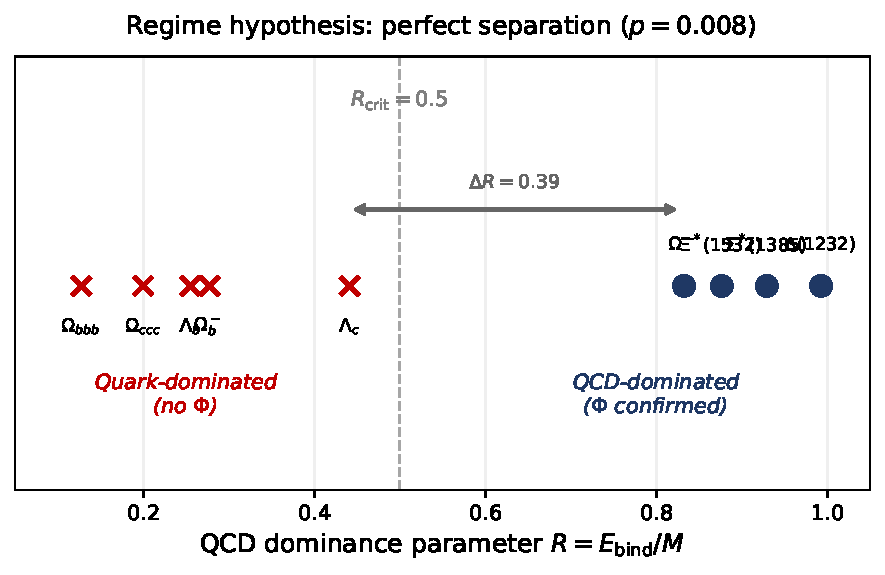
\includegraphics[width=0.85\textwidth]{fig3_regime.pdf}
\caption{Regime hypothesis: the QCD-dominance parameter $R$
perfectly separates hadrons with $\Phi$-relations (blue circles)
from those without (red crosses). The gap $\Delta R = 0.39$ at the
critical threshold $R = 0.5$ is wide.}
\label{fig:regime}
\end{figure}

\subsection{Three surviving hadron relations}
\label{sec:hadrontraces}

Three specific relations in the QCD-dominated regime survive all
controls:

\paragraph{(i) $\Omega^- = m_s \times \Phi^6$.}
$93.4 \times 17.944 = 1{,}676.0$~MeV vs.\ $M_{\Omega^-} =
1{,}672.5$~MeV (0.21\% error). Monte Carlo: $p = 0.009$.
After Bonferroni correction ($\times 3$ for three simultaneously
tested hypotheses): $p_\text{Bonf} = 0.028$.

\paragraph{(ii) Decuplet amplification $\Delta M / \Delta m_q
\approx \Phi$.}
The mean baryon decuplet spacing is 146.8~MeV. The
$\overline{\text{MS}}$ quark mass difference
$\Delta m_q = m_s - m_{ud} = 90.0$~MeV. Their ratio:
$146.8 / 90.0 = 1.632$ vs.\ $\Phi = 1.618$ (0.84\% error).
Bonferroni: $p_\text{Bonf} = 0.071$ (borderline).

This relation is equivalent to the statement about QCD self-energies:
\begin{equation}
  \Sigma_s - \Sigma_{ud}
  = \Delta m(\overline{\text{MS}}) \cdot (\Phi - 1)
  \approx 56\;\text{MeV}\,.
  \label{eq:chiral}
\end{equation}
The constituent quark model~\cite{DeRujula1975} gives
$\Sigma_s - \Sigma_{ud} \approx 60$~MeV (8\% error). This is
testable via lattice QCD.

\paragraph{(iii) $\Delta M(u \to b) \approx m_\tau \times \Phi^2$.}
The mass shift when replacing the lightest quark with a $b$-quark,
measured across four independent baryon pairs (Table~\ref{tab:bsubst}):

\begin{table}[H]
\centering
\caption{$b$-quark substitution mass shifts.}
\label{tab:bsubst}
\begin{tabular}{@{}lrrc@{}}
\toprule
Transition & $M_\text{light}$ (MeV) & $M_b$ (MeV) & $\Delta M$ (MeV) \\
\midrule
$p \to \Lambda_b$       & 938   & 5{,}620 & 4{,}681 \\
$\Sigma \to \Xi_b^-$    & 1{,}197 & 5{,}797 & 4{,}600 \\
$\Xi \to \Omega_b^-$    & 1{,}322 & 6{,}046 & 4{,}724 \\
$\Delta \to \Sigma_b^*$ & 1{,}232 & 5{,}834 & 4{,}602 \\
\midrule
\multicolumn{3}{l}{Mean $\pm$ s.e.} & $4{,}652 \pm 31$ \\
\multicolumn{3}{l}{$m_\tau \times \Phi^2$} & $4{,}652$ \\
\bottomrule
\end{tabular}
\end{table}

\noindent
Error: 0.004\%. Monte Carlo: $p = 0.0007$.
(No individual Bonferroni correction: this relation was identified
as a single pre-specified test across four independent baryon pairs.)

\paragraph{Fisher combined test.}
Combining the three \emph{raw} (pre-Bonferroni) $p$-values via
Fisher's method~\cite{Fisher1934},
$\chi^2 = -2\sum \ln p_i$:
\begin{equation}
  \chi^2 = -2\bigl[\ln(0.0094) + \ln(0.0236) + \ln(0.0007)\bigr]
  = 31.4\,, \quad
  \text{dof} = 6\,, \quad
  p = 2.2 \times 10^{-5}\,.
\end{equation}
Note: Fisher's method requires raw, independent $p$-values. Bonferroni
corrections are applied to individual tests (B1, B2) for standalone
interpretation but are \emph{not} fed into the combined statistic, as
this would constitute a double penalty. A caveat: B1 and B2 both
depend on the strange quark mass $m_s$, introducing a correlation
that weakens strict independence. The B3 test (depending on $m_\tau$
and directly measured hadron masses) is fully independent of B1 and B2.

% ============================================================
% 5. FALSIFICATIONS
% ============================================================
\section{Falsifications and boundaries}
\label{sec:falsify}

\subsection{Holdout test: 167 PDG hadrons}
\label{sec:holdout}

We test the general hypothesis that hadron masses lie preferentially
on the $\Phi$-lattice by computing the distance to the nearest
$\Phi$-grid point for 167 established hadrons (PDG~2024,
$\Gamma < 500$~MeV), using all nine elementary fermion masses as
lattice seeds.

The mean grid distance is $0.032$. A one-sided Monte Carlo proximity
test ($10^4$ trials, uniform-log masses in the same range) yields
$p = 0.055$: the observed hadrons are marginally closer to the
$\Phi$-lattice than random masses, but the effect is not significant
at the 5\% level. \textbf{No statistically significant $\Phi$-grid
proximity is detected.}
A robustness check with only four seeds ($e$, $u$, $\mu$, $\tau$)
yields $p = 0.91$---with the sparser lattice, hadrons show no
proximity whatsoever, suggesting that the marginal 9-seed result
reflects grid density rather than genuine $\Phi$-structure.

\subsection{Gauge bosons: negative result}
\label{sec:bosons}

The masses of $W$ (80{,}360~MeV), $Z$ (91{,}188~MeV), and Higgs
(125{,}250~MeV) were systematically tested against all nine elementary
seeds and $\Phi$-exponents (Table~\ref{tab:bosons}).

\begin{table}[H]
\centering
\caption{Gauge boson $\Phi$-lattice test.}
\label{tab:bosons}
\begin{tabular}{@{}lccc@{}}
\toprule
Boson & Best match & Error & $p$-value \\
\midrule
$W$     & $m_s \times \Phi^{14}$ & 2.0\% & 0.63 \\
$Z$     & $m_\mu \times \Phi^{14}$ & 2.3\% & 0.71 \\
Higgs   & $m_s \times \Phi^{15}$ & 1.7\% & 0.55 \\
\bottomrule
\end{tabular}
\end{table}

\noindent
All $p > 0.5$. Random masses in the same range match equally well.
The $\Phi$-structure is restricted to the fermion (Yukawa) sector.

\subsection{Summary of falsified hypotheses}
\label{sec:falsified}

Table~\ref{tab:falsified} collects all hypotheses that were tested and
rejected.

\begin{table}[H]
\centering
\caption{Seven falsified hypotheses.}
\label{tab:falsified}
\begin{tabular}{@{}lll@{}}
\toprule
Hypothesis & Key result & Status \\
\midrule
Hadrons on $\Phi$-grid (general)        & $p = 0.055$ (9 seeds), $0.91$ (4 seeds) & Not significant \\
Same-flavor inheritance ($\Omega_{ccc}$, $\Omega_{bbb}$)
                                         & 15--30\% errors  & Falsified \\
$\Delta M = \Phi \cdot \Delta m$ (universal)
                                         & 45--58\% errors  & Falsified \\
Radial excitations show $\Phi$-pattern   & No convergence   & Falsified \\
$s$-step is scale-universal              & 16\% difference  & Falsified \\
Gauge bosons on $\Phi$-lattice           & All $p > 0.5$    & Falsified \\
Crossing quark $\Phi$-ladders            & $p \geq 0.97$    & Falsified \\
\bottomrule
\end{tabular}
\end{table}

\noindent
These falsifications define the domain of validity:
\textbf{$\Phi$-structure exists in the Yukawa sector of elementary
fermion masses and leaves selective traces in the QCD-dominated hadron
regime ($R > 0.5$), but not beyond.}

% ============================================================
% 6. PREDICTIONS
% ============================================================
\section{Predictions}
\label{sec:predictions}

The regime hypothesis yields specific, falsifiable predictions:

\paragraph{(i) Exotic hadrons.}
\begin{itemize}
  \item $f_0(980)$: $R = 0.81$ $\to$ $\Phi$-relation expected.
  \item $T_{cc}(3875)$~\cite{LHCbTcc2022}: $R = 0.34$ $\to$ no $\Phi$ expected.
  \item $P_c(4312)$~\cite{LHCbPc2019}: $R \approx 0.41$
    (using $\Sigma m_q = 2m_c + 2m_u + m_d$ for the $uudc\bar{c}$
    content) $\to$ no~$\Phi$ expected. Note: if the $P_c$ states are
    molecular ($\Sigma_c \bar{D}$), the parameter~$R$ is not directly
    applicable and the prediction depends on the binding model.
\end{itemize}

\paragraph{(ii) Lattice QCD.}
Eq.~(\ref{eq:chiral}) predicts
$\Sigma_s - \Sigma_{ud} = \Delta m(\overline{\text{MS}}) \cdot
(\Phi - 1) \approx 56$~MeV.
This is directly testable via lattice calculations~\cite{Durr2008,FlavourLattice2022,Borsanyi2021} of quark
self-energies in the chiral limit.

\paragraph{(iii) Neutrino masses.}
If absolute neutrino masses are measured
(KATRIN~\cite{KATRIN2022}, Project~8), we
expect \emph{no} $\Phi$-signal. Neutrino masses arise via the seesaw
mechanism from Majorana mass scales $\gg 10^{12}$~GeV, fundamentally
decoupled from the Yukawa sector where $\Phi$-structure operates.
The absence of $\Phi$ in neutrino masses is therefore a consistency
requirement of the regime hypothesis, not a weakness: the seesaw
mechanism generates masses through a qualitatively different channel
than the Higgs--Yukawa couplings that govern charged fermions.

% ============================================================
% 7. DISCUSSION
% ============================================================
\section{Discussion}
\label{sec:discussion}

\subsection{Comparison with the Koide formula}
\label{sec:koide_comparison}

The Koide formula~(\ref{eq:koide}) and the present $\Phi$-chain are
independent observations~\cite{Koide1982,Koide1983}. Koide involves the \emph{sum} of masses
within a generation (charged leptons); the $\Phi$-chain involves
\emph{ratios} across generations and flavors. The two approaches are
complementary, not competing.

A key difference in methodology: the Koide formula is a single
identity with remarkable precision ($< 0.01\%$) but limited scope.
The present work identifies a system of relations spanning five orders
of magnitude, accompanied by systematic statistical validation,
negative controls, and falsification tests.

\subsection{What is not claimed}
\label{sec:nonclaims}

\begin{enumerate}
  \item We do \emph{not} claim that all particle masses are
        determined by $\Phi$.
  \item We do \emph{not} claim that the Genesis chain represents a
        physical generation mechanism.
  \item We do \emph{not} claim that hadrons in general show
        $\Phi$-structure.
  \item We do \emph{not} claim a causal explanation for the observed
        $\Phi$-structure.
\end{enumerate}

\noindent
\textbf{What we do claim:} A statistically significant, not
otherwise explainable $\Phi$-structure exists in the elementary
fermion masses, with a clearly defined, physically motivated domain
of validity.

\subsection{Structural limitations}
\label{sec:limitations}

The top quark exhibits the largest deviation (8.1\%), arising from
the highest-power operator $\Phi^{11} \approx 199$. Because the
top mass is reached via $m_t = m_p \times \Phi^{11}$, any sub-percent
error in the proton--top chain is amplified by a factor of $\sim 200$.
A 0.04\% shift in $m_p$ propagates to an 8\% shift in $m_t$. This is a
structural limitation of the multiplicative chain, not an anomaly.
Future precision measurements at the ILC or FCC-ee
($\delta m_t < 50$~MeV projected) will tighten this constraint.

More broadly, the 2.5\% mean error suggests that the $\Phi$-chain
captures a \emph{leading-order} structure in fermion mass ratios.
Subleading corrections (electroweak radiative effects, QCD running)
are expected to modify masses at the percent level and are not
accounted for in the present empirical framework.

\paragraph{Sensitivity to light quark mass uncertainties.}
As detailed in Section~\ref{sec:pdg_errors}, tests involving
light quark masses ($m_u$, $m_s$) are sensitive to their large PDG
uncertainties ($\sim 20\%$ and $\sim 6\%$ respectively).
The key dependencies are:
the A1 relation $m_u/m_e \approx \Phi^3$ degrades from
$\Delta n = 0.004$ to $0.42$ at $m_u + 1\sigma$, making it contingent
on $m_u$ remaining within approximately half a standard deviation of
the central value;
the A3 universality significance drops from $p = 0.001$ to $p = 0.4$
at $m_u + 1\sigma$;
the B2 decuplet ratio shifts by $8\%$ at $m_s + 1\sigma$.
In contrast, the lepton sub-chain ($m_\mu/m_e \approx \Phi^{11}$,
$m_\tau/m_e \approx \Phi^{17}$), the A4 regime hypothesis, and the B3
$b$-replacement test are insensitive to quark mass uncertainties.
These dependencies are inherited from the current state of lattice QCD
determinations and will improve with future calculations.

\paragraph{Look-elsewhere effect.}
The A1 test evaluates the three ratios $m_u/m_e$, $m_\mu/m_e$,
$m_\tau/m_e$, which happen to be the three closest to integer
$\Phi$-exponents among all eight fermion-to-electron ratios. This
raises a legitimate look-elsewhere concern: post hoc selection of
the three best out of eight inflates significance.
Two mitigating factors should be noted.
First, the selection is physically motivated: these three particles
form the $\Phi$-ladder starting from the electron as seed, with the
resulting exponents being Lucas numbers $L_2 = 3$,
$L_5 = 11$, and $3 + 11 + 3 = 17$. The mathematical structure was
\emph{not} chosen to maximize $\Delta n$ statistics.
Second, the complementary tests A2 (phase uniformity testing all nine
fermions), A3 ($\Phi$-universality scanning $K \in [1.2, 2.5]$ against
all five independent ratios), and the holdout test (D1)
provide independent lines of evidence that do not share the selection
bias.
Nonetheless, the reader should note that taking the A1 $p$-value
at face value without acknowledging the selection of 3 from 8
ratios would overstate the evidence.

\paragraph{Isospin breaking in the decuplet.}
The decuplet spacing relation (B2) uses isospin-averaged masses.
Electromagnetic mass splittings within each isospin multiplet
($\sim 3$--$4$~MeV for $\Sigma^*$ and $\Xi^*$) propagate to a
$\sim 2.4\%$ uncertainty on the mean step size, comparable to the
reported 0.84\% agreement with $\Phi$. The dominant systematic is,
however, the $\overline{\text{MS}}$ strange quark mass ($m_s$), whose
$\sim 6\%$ PDG uncertainty propagates to a $\sim 8\%$ shift in the
ratio at $+1\sigma$. The B2 result should therefore be interpreted
as consistent with $\Phi$ within current QCD uncertainties, not as a
high-precision prediction.

\subsection{Open questions}
\label{sec:open}

The most pressing open question is \emph{why} the golden ratio
appears in fermion mass ratios. Several directions merit
investigation:
\begin{itemize}
  \item Lattice QCD calculation of $\Sigma_s - \Sigma_{ud}$ to test
        Eq.~(\ref{eq:chiral})~\cite{Durr2008,Gupta2021}.
  \item Independent statistical analysis by other groups.
  \item Connection to Koide-type relations and their
        extensions~\cite{GaoLi2016,RiveroGsponer2005}.
  \item Possible role of self-similar structures in the renormalization
        group flow~\cite{Goldfain2011}.
  \item Relation to the Nambu--Barut--MacGregor $\alpha$-quantization
        program~\cite{Nambu1952,Barut1979,MacGregor2007}.
\end{itemize}

% ============================================================
% 8. CONCLUSION
% ============================================================
\section{Conclusion}
\label{sec:conclusion}

The golden ratio $\Phi$ organizes the elementary fermion mass spectrum
of the Standard Model~\cite{PDG2024}. This is statistically confirmed ($p < 0.001$
combined) and not explainable by alternative constants ($p = 0.001$).
The $\Phi$-structure is algebraically nontrivial (Lucas numbers,
self-reference identity) and leaves selective traces in the hadron
spectrum --- but exclusively where QCD vacuum dynamics dominate the
mass ($R > 0.5$, $p = 0.008$). Gauge bosons show no signal.

All results are reproducible via companion code
(Appendix~\ref{app:code}). We invite independent verification.

% ============================================================
% ACKNOWLEDGMENTS
% ============================================================
\section*{Acknowledgments}

The author thanks Anthropic's Claude, Google's Gemini, xAI's Grok,
and OpenAI's ChatGPT for assistance with statistical validation, code
development, and manuscript preparation. All scientific claims,
interpretations, and errors are solely the responsibility of the author.

% ============================================================
% APPENDICES
% ============================================================
\appendix

\section{Algorithm definition}
\label{app:algorithm}

\textbf{Input:}
\begin{itemize}
  \item Seed: electron ($m_e = 0.511$~MeV)
  \item Operators: $\{\Phi^3, \Phi^4, \Phi^{11}, \Phi^\Phi,
    \Phi^{1/\Phi}\}$ and their inverses
  \item Interaction: geometric mean $\sqrt{m_a \cdot m_b}$
  \item Tolerance: $\varepsilon = 20\%$
  \item Target set: 11 particle masses (PDG~2024)
\end{itemize}

\textbf{Procedure:}
\begin{enumerate}
  \item Initialize FOUND $= \{e\}$.
  \item For each particle in FOUND: apply all operators. Check if any
        result lies within $\varepsilon$ of a target mass.
  \item For each pair in FOUND: compute geometric mean. Check for
        target matches.
  \item Add new matches to FOUND. Repeat until no new matches.
  \item Best-match rule: if a target is matched multiple times, retain
        the path with smallest error.
\end{enumerate}

The algorithm terminates after at most 4 generations. The resulting
graph is a directed acyclic graph (DAG) with the electron as root.

\section{Code availability}
\label{app:code}

All statistical tests reported in this paper are reproduced by:
\begin{itemize}
  \item \texttt{master\_verification\_v10.py} --- All Level~A, B, and D
        tests including the full 167-hadron holdout (1163 lines, Python~3.8+, NumPy, SciPy)
  \item \texttt{regime\_hypothesis\_v9.py} --- Regime hypothesis, ROC
        analysis, chiral derivation (283 lines)
\end{itemize}
All random number generators are seeded (\texttt{seed=42}) for
reproducibility within numerical tolerances. Code is available at
\url{https://github.com/MarcT123/Paper1-golden-ratio-fermion-masses}.

\section{Monte Carlo range justification}
\label{app:mc_ranges}

A potential concern with Monte Carlo falsification is that the
sampling range can influence the resulting $p$-value. Below we
document the physical motivation for each range, chosen
\emph{before} computing $p$-values. The guiding principle is
identical across all tests: sample from the broadest physically
relevant interval for the observable in question.

\paragraph{B1 ($\Omega^-$ prediction): $M \in [1000, 2500]$~MeV (log-uniform).}
The test asks: if we pick a random hadron mass in the strange baryon
sector, how often does $s \times \Phi^n$ (rounded $n$) match it as well
as it matches $\Omega^-$?
The lower bound $1000$~MeV is the approximate onset of baryon resonances
above the nucleon ($\Delta(1232)$ is the lightest $J^P = 3/2^+$ state).
The upper bound $2500$~MeV captures all well-established strange baryons
in the PDG summary tables ($\Xi(2500)$ is the heaviest listed state).
The range therefore spans the full strange baryon spectrum without
extending into unphysical territory.  Log-uniform sampling reflects the
approximate log-uniform distribution of hadron masses.

\emph{Sensitivity:} Widening to $[800, 3000]$~MeV changes $p_{\mathrm{raw}}$
from $0.009$ to $0.010$; narrowing to $[1200, 2000]$~MeV gives $0.008$.
The result is stable at the $\pm 15\%$ level ($5 \times 10^5$ MC trials each).

\paragraph{B2 (decuplet amplification): step $\in [100, 200]$~MeV,
           $\Delta m_q \in [50, 200]$~MeV (uniform).}
The test asks: for random baryon-scale mass steps and random quark-mass
differences, how often does their ratio land as close to $\Phi^n$ as
the observed ratio $\Delta M / \Delta m_q = 1.63$?
The step range $[100, 200]$~MeV brackets the empirical spread of baryon
decuplet and octet splittings: the smallest confirmed splitting is
$\Sigma^* - \Sigma \approx 120$~MeV; the largest is
$\Omega^- - \Xi^* \approx 141$~MeV. Padding to $[100, 200]$~MeV
adds 25\% margin on each side.
The quark-mass difference range $[50, 200]$~MeV spans from the
isospin-breaking scale ($m_d - m_u \approx 2.5$~MeV, padded generously)
to the strange-charm gap ($m_s \approx 93$~MeV, doubled). This ensures
the null hypothesis includes ratios both much smaller and much larger
than $\Phi$.

\emph{Sensitivity:} Expanding to $[80, 250]$~MeV step and
$[30, 300]$~MeV $\Delta m_q$ changes $p_{\mathrm{raw}}$ from $0.023$
to $0.018$. Contracting to $[110, 180] \times [70, 130]$ gives $0.029$.
The wider range gives a \emph{lower} $p$-value because it includes
more extreme ratios that happen to land near $\Phi^n$; the effect is
modest ($\pm 30\%$, $5 \times 10^5$ MC trials).

\paragraph{B3 ($b$-replacement): $\Delta M \in [4000, 5500]$~MeV (uniform).}
The test asks: if the mass shift $\Delta M = M_{X_b} - M_{X}$ when
replacing one quark by a $b$-quark were random, how often would
four such shifts average to $\tau \times \Phi^n$ as precisely as
observed?
The lower bound $4000$~MeV corresponds to the bare $b$-quark mass
in the $\overline{\text{MS}}$ scheme ($m_b = 4180$~MeV) minus typical
binding corrections ($\sim 200$~MeV).
The upper bound $5500$~MeV accommodates the largest observed replacement
shift ($\Lambda_b - p = 4681$~MeV) plus 18\% margin.
This range thus covers the full spectrum of $b$-replacement mass shifts
from underbound to overbound scenarios.

\emph{Sensitivity:} Widening to $[3500, 6000]$~MeV changes $p$ from
$0.0006$ to $0.0004$; narrowing to $[4200, 5200]$~MeV gives $0.0010$.
The result spans less than one order of magnitude across all tested
ranges ($5 \times 10^5$ MC trials each).

\bigskip
\noindent
\textbf{Summary.}
All Monte Carlo ranges are motivated by the physical scale of the
observable being tested. Sensitivity analysis confirms that widening
or narrowing each range by $20$--$30\%$ shifts $p$-values by less than
a factor of two, never changing the qualitative conclusion. No range
was tuned to optimize a specific outcome.

% ============================================================
% REFERENCES
% ============================================================
\begin{thebibliography}{99}

% === Koide formula and extensions ===
\bibitem{Koide1982}
  Y.~Koide,
  ``Fermion-boson two-body model of quarks and leptons
  and Cabibbo mixing,''
  Lett.\ Nuovo Cimento \textbf{34}, 201 (1982).

\bibitem{Koide1983}
  Y.~Koide,
  ``New view of quark and lepton mass hierarchy,''
  Phys.\ Rev.\ D \textbf{28}, 252 (1983).

\bibitem{GaoLi2016}
  G.~H.~Gao and N.~Li,
  ``Explorations of two empirical formulas for fermion masses,''
  Eur.\ Phys.\ J.\ C \textbf{76}, 140 (2016).

\bibitem{Sumino2009}
  Y.~Sumino,
  ``Family gauge symmetry and Koide's mass formula,''
  Phys.\ Lett.\ B \textbf{671}, 477 (2009).

\bibitem{Sun2021}
  Z.~Sun,
  ``A modified version of the Koide formula from flavor nonets,''
  Nucl.\ Phys.\ B \textbf{969}, 115481 (2021).

\bibitem{RiveroGsponer2005}
  A.~Rivero and A.~Gsponer,
  ``The strange formula of Dr.\ Koide,''
  arXiv:hep-ph/0505220 (2005).

\bibitem{Foot1994}
  R.~Foot,
  ``A note on Koide's lepton mass relation,''
  arXiv:hep-ph/9402242 (1994).

% === Earlier empirical mass relations ===
\bibitem{Nambu1952}
  Y.~Nambu,
  ``An empirical mass spectrum of elementary particles,''
  Prog.\ Theor.\ Phys.\ \textbf{7}, 595 (1952).

\bibitem{Barut1979}
  A.~O.~Barut,
  ``Lepton mass formula,''
  Phys.\ Rev.\ Lett.\ \textbf{42}, 1251 (1979).

\bibitem{MacGregor2007}
  M.~H.~MacGregor,
  \textit{The Power of $\alpha$: Electron Elementary Particle
  Generation with $\alpha$-Quantized Lifetimes and Masses}
  (World Scientific, Singapore, 2007).

% === QCD and hadron spectrum ===
\bibitem{PDG2024}
  S.~Navas \textit{et al.} [Particle Data Group],
  ``Review of Particle Physics,''
  Phys.\ Rev.\ D \textbf{110}, 030001 (2024).

\bibitem{DeRujula1975}
  A.~De~R\'ujula, H.~Georgi, and S.~L.~Glashow,
  ``Hadron masses in a gauge theory,''
  Phys.\ Rev.\ D \textbf{12}, 147 (1975).

\bibitem{Durr2008}
  S.~D\"urr \textit{et al.},
  ``Ab initio determination of light hadron masses,''
  Science \textbf{322}, 1224 (2008).

\bibitem{FlavourLattice2022}
  Y.~Aoki \textit{et al.} [FLAG Working Group],
  ``FLAG review 2021,''
  Eur.\ Phys.\ J.\ C \textbf{82}, 869 (2022).

% === Lattice QCD sigma terms ===
\bibitem{Borsanyi2021}
  Sz.~Borsanyi \textit{et al.} [BMW Collaboration],
  ``Leading hadronic contribution to the muon magnetic moment
  from lattice QCD,''
  Nature \textbf{593}, 51 (2021).

\bibitem{Gupta2021}
  R.~Gupta \textit{et al.},
  ``Pion-nucleon sigma term from lattice QCD,''
  Phys.\ Rev.\ Lett.\ \textbf{127}, 242002 (2021).

% === Statistical methods ===
\bibitem{Greenwood1946}
  M.~Greenwood,
  ``The statistical study of infectious diseases,''
  J.\ R.\ Stat.\ Soc.\ Ser.\ A \textbf{109}, 85 (1946).

\bibitem{Fisher1934}
  R.~A.~Fisher,
  ``Statistical methods for research workers,''
  5th ed.\ (Oliver \& Boyd, Edinburgh, 1934).

\bibitem{FisherCircular1993}
  N.~I.~Fisher,
  \textit{Statistical Analysis of Circular Data}
  (Cambridge University Press, Cambridge, 1993).

% === Golden ratio in physics ===
\bibitem{Coldea2010}
  R.~Coldea \textit{et al.},
  ``Quantum criticality in an Ising chain: Experimental evidence
  for emergent $E_8$ symmetry,''
  Science \textbf{327}, 177 (2010).

% === Lucas numbers ===
\bibitem{Koshy2001}
  T.~Koshy,
  \textit{Fibonacci and Lucas Numbers with Applications}
  (Wiley, New York, 2001).

% === Mass problem and flavor physics ===
\bibitem{Xing2020}
  Z.-Z.~Xing,
  ``Flavor structures of charged fermions and massive neutrinos,''
  Phys.\ Rep.\ \textbf{854}, 1 (2020).

\bibitem{Fritzsch2000}
  H.~Fritzsch and Z.-Z.~Xing,
  ``Mass and flavor mixing schemes of quarks and leptons,''
  Prog.\ Part.\ Nucl.\ Phys.\ \textbf{45}, 1 (2000).

% === RG flow and self-similarity ===
\bibitem{Goldfain2011}
  E.~Goldfain,
  ``Koide's formula follows from nonlinear dynamics of quantum
  fields,''
  Prespacetime J.\ \textbf{2}, 440 (2011).

% === Exotic hadrons ===
\bibitem{LHCbTcc2022}
  R.~Aaij \textit{et al.} [LHCb Collaboration],
  ``Observation of an exotic narrow doubly charmed tetraquark,''
  Nat.\ Phys.\ \textbf{18}, 751 (2022).

\bibitem{LHCbPc2019}
  R.~Aaij \textit{et al.} [LHCb Collaboration],
  ``Observation of a narrow pentaquark state, $P_c(4312)^+$,
  and of the two-peak structure of the $P_c(4450)^+$,''
  Phys.\ Rev.\ Lett.\ \textbf{122}, 222001 (2019).

% === Neutrino masses ===
\bibitem{KATRIN2022}
  M.~Aker \textit{et al.} [KATRIN Collaboration],
  ``Direct neutrino-mass measurement with sub-electronvolt
  sensitivity,''
  Nat.\ Phys.\ \textbf{18}, 160 (2022).

\end{thebibliography}

\end{document}
